\begin{center}
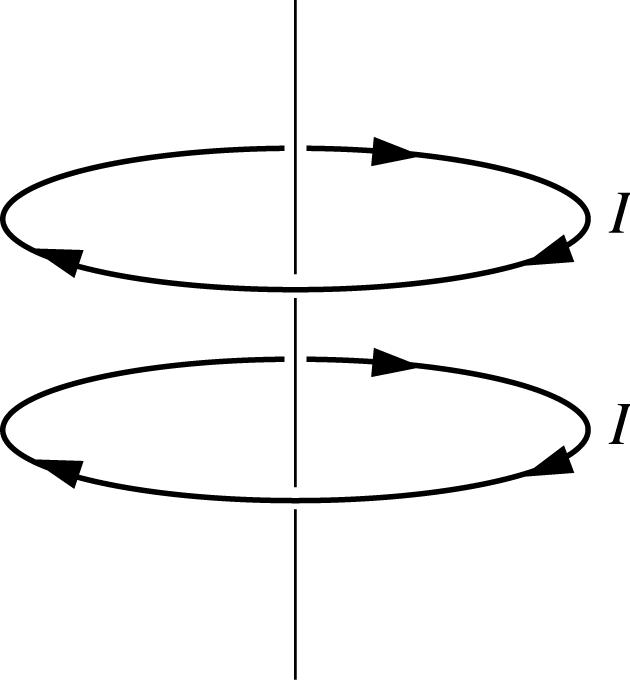
\includegraphics[scale=0.25]{images/img-011-023.png}
\end{center}

% Multiple Choice Question 20
\begin{questions}\setcounter{question}{19}\question
Two conducting loops that are centered on the same axis carry equal currents $I$ in the same direction as shown in the diagram above. If the current in the upper loop suddenly decreases to zero, what happens to the current in the lower loop according to Lenz's law?

\begin{choices}
\choice It also decreases to zero.
\choice It decreases, but not to zero.
\choice It does not change.
\choice It increases.
\choice Its direction is reversed.
\end{choices}\end{questions}

